% THIS DOCUMENT IS FOLLOWS THE VOLERE TEMPLATE BY Suzanne Robertson and James Robertson
% ONLY THE SECTION HEADINGS ARE PROVIDED
%
% Initial draft from https://github.com/Dieblich/volere
%
% Risks are removed because they are covered by the Hazard Analysis
\documentclass[12pt]{article}
\usepackage{graphicx}
\usepackage{booktabs}
\usepackage{tabularx}
\usepackage{hyperref}
\hypersetup{
    bookmarks=true,         % show bookmarks bar?
      colorlinks=true,      % false: boxed links; true: colored links
    linkcolor=red,          % color of internal links (change box color with linkbordercolor)
    citecolor=green,        % color of links to bibliography
    filecolor=magenta,      % color of file links
    urlcolor=cyan           % color of external links
}

\newcommand{\lips}{\textit{Insert your content here.}}

%% Comments

\usepackage{color}

\newif\ifcomments\commentstrue %displays comments
%\newif\ifcomments\commentsfalse %so that comments do not display

\ifcomments
\newcommand{\authornote}[3]{\textcolor{#1}{[#3 ---#2]}}
\newcommand{\todo}[1]{\textcolor{red}{[TODO: #1]}}
\else
\newcommand{\authornote}[3]{}
\newcommand{\todo}[1]{}
\fi

\newcommand{\wss}[1]{\authornote{magenta}{SS}{#1}} 
\newcommand{\plt}[1]{\authornote{cyan}{TPLT}{#1}} %For explanation of the template
\newcommand{\an}[1]{\authornote{cyan}{Author}{#1}}

%% Common Parts

\newcommand{\progname}{SFWRENG 4G06 - Capstone Design Process}
\newcommand{\authname}{\textbf{Team 17, DomainX} \\
\\ Awurama Nyarko
\\ Haniye Hamidizadeh
\\ Fei Xie
\\ Ghena Hatoum             
}
\usepackage{hyperref}
    \hypersetup{colorlinks=true, linkcolor=blue, citecolor=blue, filecolor=blue,
                urlcolor=blue, unicode=false}
    \urlstyle{same}
                                


\begin{document}

\title{Software Requirements Specification for \progname: subtitle describing software} 
\author{\authname}
\date{\today}
	
\maketitle

\pagenumbering{roman}
\begin{table}[hp]
\caption{Revision History} \label{TblRevisionHistory}
\begin{tabularx}{\textwidth}{llX}
\toprule
\textbf{Date} & \textbf{Developer(s)} & \textbf{Change}\\
\midrule
October 6, 2025 & Fei Xie & First Draft of Sections: Cost to Ideas for Solution\\
Date2 & Name(s) & Description of changes\\
... & ... & ...\\
\bottomrule
\end{tabularx}
\end{table}

~\newpage

\tableofcontents

~\newpage
\section{Purpose of the Project}
\subsection{User Business}
\lips
\subsection{Goals of the Project}
\lips
\section{Stakeholders}
\subsection{Client}
\lips
\subsection{Customer}
\lips
\subsection{Other Stakeholders}
\lips
\subsection{Hands-On Users of the Project}
\lips
\subsection{Personas}
\lips
\subsection{Priorities Assigned to Users}
\lips
\subsection{User Participation}
\lips
\subsection{Maintenance Users and Service Technicians}
\lips

\section{Mandated Constraints}
\subsection{Solution Constraints}
\lips
\subsection{Implementation Environment of the Current System}
\lips
\subsection{Partner or Collaborative Applications}
\lips
\subsection{Off-the-Shelf Software}
\lips
\subsection{Anticipated Workplace Environment}
\lips
\subsection{Schedule Constraints}
\lips
\subsection{Budget Constraints}
\lips
\subsection{Enterprise Constraints}
\lips

\section{Naming Conventions and Terminology}
\subsection{Glossary of All Terms, Including Acronyms, Used by Stakeholders
involved in the Project}
\lips

\section{Relevant Facts And Assumptions}
\subsection{Relevant Facts}
\lips
\subsection{Business Rules}
\lips
\subsection{Assumptions}
\lips

\section{The Scope of the Work}
\subsection{The Current Situation}
\lips
\subsection{The Context of the Work}
\lips
\subsection{Work Partitioning}
\lips
\subsection{Specifying a Business Use Case (BUC)}
\lips

\section{Business Data Model and Data Dictionary}
\subsection{Business Data Model}
\lips
\subsection{Data Dictionary}
\lips

\section{The Scope of the Product}
\subsection{Product Boundary}
\lips
\subsection{Product Use Case Table}
\lips
\subsection{Individual Product Use Cases (PUC's)}
\lips

\section{Functional Requirements}
\subsection{Functional Requirements}
\lips

\section{Look and Feel Requirements}
\subsection{Appearance Requirements}
\lips
\subsection{Style Requirements}
\lips

\section{Usability and Humanity Requirements}
\subsection{Ease of Use Requirements}
\lips
\subsection{Personalization and Internationalization Requirements}
\lips
\subsection{Learning Requirements}
\lips
\subsection{Understandability and Politeness Requirements}
\lips
\subsection{Accessibility Requirements}
\lips

\section{Performance Requirements}
\subsection{Speed and Latency Requirements}
\lips
\subsection{Safety-Critical Requirements}
\lips
\subsection{Precision or Accuracy Requirements}
\lips
\subsection{Robustness or Fault-Tolerance Requirements}
\lips
\subsection{Capacity Requirements}
\lips
\subsection{Scalability or Extensibility Requirements}
\lips
\subsection{Longevity Requirements}
\lips

\section{Operational and Environmental Requirements}
\subsection{Expected Physical Environment}
\lips
\subsection{Wider Environment Requirements}
\lips
\subsection{Requirements for Interfacing with Adjacent Systems}
\lips
\subsection{Productization Requirements}
\lips
\subsection{Release Requirements}
\lips

\section{Maintainability and Support Requirements}
\subsection{Maintenance Requirements}
\lips
\subsection{Supportability Requirements}
\lips
\subsection{Adaptability Requirements}
\lips

\section{Security Requirements}
\subsection{Access Requirements}
\lips
\subsection{Integrity Requirements}
\lips
\subsection{Privacy Requirements}
\lips
\subsection{Audit Requirements}
\lips
\subsection{Immunity Requirements}
\lips

\section{Cultural Requirements}
\subsection{Cultural Requirements}
\lips

\section{Compliance Requirements}
\subsection{Legal Requirements}
\lips
\subsection{Standards Compliance Requirements}
\lips

\section{Open Issues}
\lips

\section{Off-the-Shelf Solutions}
\subsection{Ready-Made Products}
\lips
\subsection{Reusable Components}
\lips
\subsection{Products That Can Be Copied}
\lips

\section{New Problems}
\subsection{Effects on the Current Environment}
\lips
\subsection{Effects on the Installed Systems}
\lips
\subsection{Potential User Problems}
\lips
\subsection{Limitations in the Anticipated Implementation Environment That May
Inhibit the New Product}
\lips
\subsection{Follow-Up Problems}
\lips

\section{Tasks}
\subsection{Project Planning}
\lips
\subsection{Planning of the Development Phases}
\lips

\section{Migration to the New Product}
\subsection{Requirements for Migration to the New Product}
\lips
\subsection{Data That Has to be Modified or Translated for the New System}
\lips

\section{Costs}
There is no development cost for this project, due to the nature of this being a capstone project. 
\\
The costs of hosting the required services, such as the database and the web application will depend on McMaster University's existing infrastructure.
\\
However, estimating using a common cloud provider such as Amazon Web Services (AWS). \\
Using the Relational Database Service (RDS) for database and the Elastic Cloud Computing (EC2) service for hosting.
Assuming around a maximum usage of 20 Hours/Month, the total cost of hosting is 11.63 CAD per month, as shown in Table~\ref{tab:price_table}.
\begin{table}[h!]
\centering
\begin{tabularx}{\textwidth}{@{} X X X c @{}}
\toprule
\textbf{Name} & \textbf{Configuration} & \textbf{Estimated Usage} & \textbf{Total Cost} \\
\midrule
RDS for MySQL & Two vCPU and 8GB of Memory & 20 Hours/Month & 9.76 CAD/Month \\ 
EC2 & t4g.large Instance & 20 Hours/Month & 1.87 USD/Month \\
\bottomrule
\end{tabularx}
\caption{Price estimates and total costs for two AWS services.}
\label{tab:price_table}
\end{table}

\section{User Documentation and Training}
\subsection{User Documentation Requirements}
\subsubsection{User Manual}
The user manual will highlight the key features of the product, and provide additional details for installing, setup and usage that wasn't previously covered in the project's \href{https://github.com/thaafei/DomainX/blob/main/README.md}{README}. \\
\\The maintenance of this document will be the responsibility of the development team. Changes to the product's features, such as adding new features or altering existing features must be reflected in the user manual upon release of the update.

\subsubsection{Release Manual}
The release manual will cover the release process required for future releases of the product, found in the \href{https://github.com/thaafei/DomainX/blob/main/docs/DevelopmentPlan/DevelopmentPlan.pdf}{Development Plan}. It should include the whole CI/CD lifecycle, including team standards, release labelling, and more.\\
\\The maintenance of this document will be the responsibility of the development team. Changes to the CI/CD process, either from the development team or the broader McMaster University infrastructure team should be reflected before the next release.

\subsection{Training Requirements}
\textbf{1. Users should be able to use the tool and utilize key features immediately after following the tutorial} \\ \\
\textbf{2. Users should be able to find key features without consulting additional documentation 95\% of the time.} \\ \\
The responsibilty of the training will first fall towards the development team of the tool. They must ensure the provided in-tool tutorial is up-to-date and sufficient to help a user understand all key features.
\\ Additional training will be provided to the supervisor, hosted by the development team.
Subsequent training will be the responsibility of the supervisor, if needed to train future users of the tool, in the format that the supervisor chooses.
\section{Waiting Room}
\textbf{1. Comparing across Domains}\\
The user should be able to compare two (or more) completed domain analysis against each other. \\\\
\textbf{2. Versioning of Domains}\\
Users can revist and update completed domains, adding new data or editing existing ones. Allowing users to view the evolution of the state of best practice for the domain.

\section{Ideas for Solution}
The following is the development team's idea for the user interface of the tool. Figure~\ref{fig:domainx_ui} shows the initial concept, drawing inspiration from \href{https://octave-online.net/}{Octave Online}, the cloud IDE for Matlab.
\\ The main section of the tool will be where the data is displayed and gathered for each domain. With the sections that can be automatically gathered differentiated using a different colour, such as the gray shown in Figure~\ref{fig:domainx_ui}.
\\ The left sidebar will contain all the domains, with indications on whether it's completed or not. As well as providing a filter to quickly search for a specific domain.
\begin{figure}
\centering
  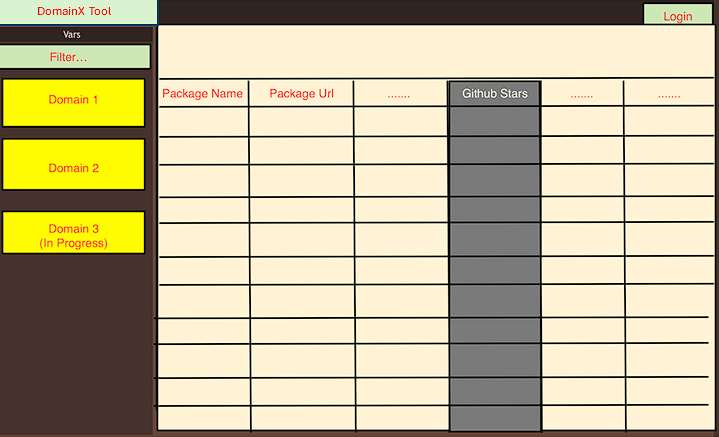
\includegraphics[totalheight=8cm]{images/DomainX-UI.png}
  \caption{DomainX UI, inspired by Octave Online}
  \label{fig:domainx_ui}
\end{figure}
\newpage{}
\section*{Appendix --- Reflection}

The purpose of reflection questions is to give you a chance to assess your own
learning and that of your group as a whole, and to find ways to improve in the
future. Reflection is an important part of the learning process.  Reflection is
also an essential component of a successful software development process.  

Reflections are most interesting and useful when they're honest, even if the
stories they tell are imperfect. You will be marked based on your depth of
thought and analysis, and not based on the content of the reflections
themselves. Thus, for full marks we encourage you to answer openly and honestly
and to avoid simply writing ``what you think the evaluator wants to hear.''

Please answer the following questions.  Some questions can be answered on the
team level, but where appropriate, each team member should write their own
response:


\begin{enumerate}
  \item What went well while writing this deliverable? 
  \item What pain points did you experience during this deliverable, and how did
  you resolve them?
  \item How many of your requirements were inspired by speaking to your
  client(s) or their proxies (e.g. your peers, stakeholders, potential users)?
  \item Which of the courses you have taken, or are currently taking, will help
  your team to be successful with your capstone project.
  \item What knowledge and skills will the team collectively need to acquire to
  successfully complete this capstone project?  Examples of possible knowledge
  to acquire include domain specific knowledge from the domain of your
  application, or software engineering knowledge, mechatronics knowledge or
  computer science knowledge.  Skills may be related to technology, or writing,
  or presentation, or team management, etc.  You should look to identify at
  least one item for each team member.
  \item For each of the knowledge areas and skills identified in the previous
  question, what are at least two approaches to acquiring the knowledge or
  mastering the skill?  Of the identified approaches, which will each team
  member pursue, and why did they make this choice?
\end{enumerate}


\end{document}